\begin{figure}[!htbp]

\begin{center}
\begin{subfigure}[b]{\linewidth}
  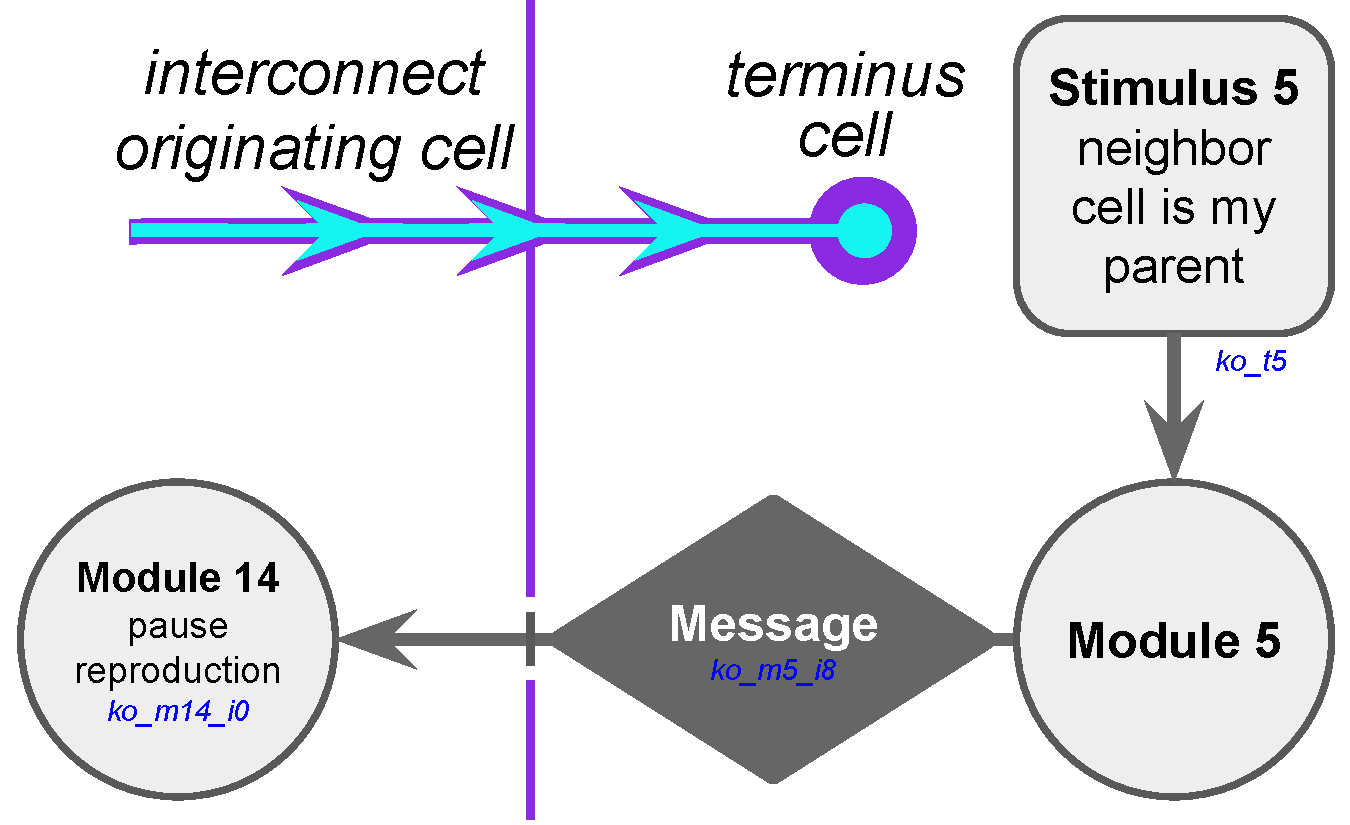
\includegraphics[width=\linewidth,clip]{batch=2032+step=1018+pop=0/2032_diagram}
  \caption{Hypothesized selective reproduction pausing mechanism}
  \label{fig:mechanism2}
\end{subfigure}
\begin{subfigure}[b]{0.45\linewidth}
  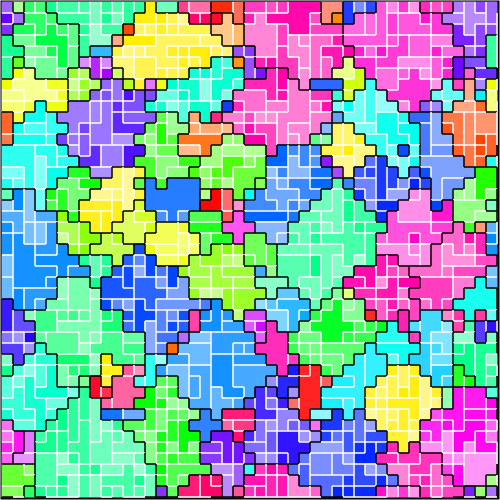
\includegraphics[width=\linewidth,trim={0 200 200 0},clip]{batch=2032+step=1018+pop=0/seed=1+title=channel+treat=batch_2032,step_1018,pop_1,id1_wt+update=5000+_emp_hash=0c549f0-clean+_source_hash=d50b431-dirty+ext=}
  \caption{Kin groups}
  \label{fig:kingroups2}
\end{subfigure}
\begin{subfigure}[b]{0.45\linewidth}
  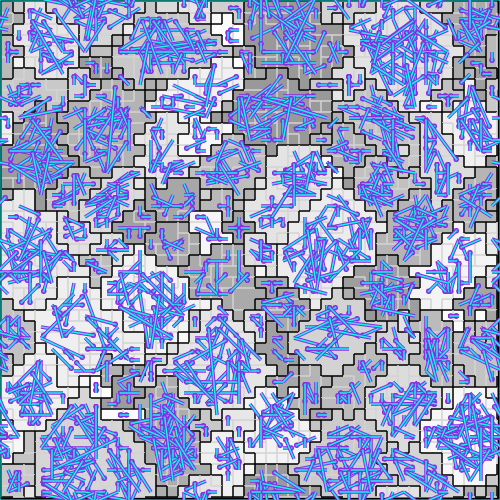
\includegraphics[width=\linewidth,trim={0 200 200 0},clip]{batch=2032+step=1018+pop=0/seed=1+title=established-interconnect+treat=batch_2032,step_1018,pop_1,id1_wt+update=5000+_emp_hash=0c549f0-clean+_source_hash=d50b431-dirty+ext=}
  \caption{Established interconnects}
  \label{fig:establishedinterconnects2}
\end{subfigure}
\begin{subfigure}[b]{0.45\linewidth}
  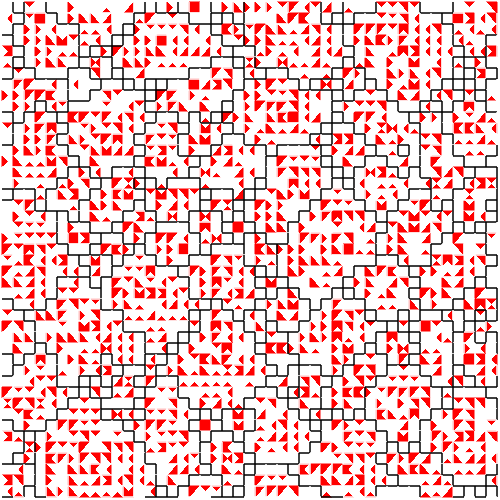
\includegraphics[width=\linewidth,trim={0 200 200 0},clip]{batch=2032+step=1018+pop=0/seed=1+title=parent-cell-of+treat=batch_2032,step_1018,pop_1,id1_wt+update=5000+_emp_hash=0c549f0-clean+_source_hash=d50b431-dirty+ext=}
  \caption{Spatial distriubiton of stimulus 5TODO fix}
  \label{fig:t5distribution}
\end{subfigure}
\begin{subfigure}[b]{0.45\linewidth}
  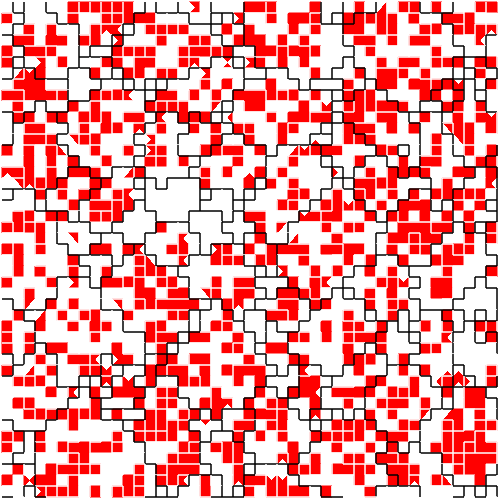
\includegraphics[width=\linewidth,trim={0 200 200 0},clip]{batch=2032+step=1018+pop=0/seed=1+title=reproductive-pause-level-0+treat=batch_2032,step_1018,pop_1,id1_wt+update=5000+_emp_hash=0c549f0-clean+_source_hash=d50b431-dirty+ext=}
  \caption{Spatial distribution of module 14 execution}
  \label{fig:m14distribution}
\end{subfigure}
\caption{
Batch 2032 case study overview.
Figures \ref{fig:kingroups2} through \ref{fig:m14distribution} are generated from a snapshot of a wild-type strain monoculture population.
In these images, each grid tile represents an individual cell.
Cells are organized into kin groups, color-coded by hue in Figure \ref{fig:kingroups2}.
Established interconnects are overlaid in blue on Figure \ref{fig:establishedinterconnects2}.
In Figures \ref{fig:t5distribution} and \ref{fig:m14distribution}, kin groups are outlined in black.
Figure \ref{fig:t5distribution} highlights cells that are sending resource over-interconnect.
Figure \ref{fig:m14distribution} highlights cells that are receiving resource over-interconnect.
You can view an animation of the wild-type monoculutre at \url{https://mmore500.com/hopto/an}.
}
\label{fig:case_study_2032}
\end{center}
\end{figure}
